%% !TeX root = report.tex

W ramach projektu została stworzona aplikacja przeprowadzająca testy
algorytmu i wizualizująca wyniki kodowania. Jedną z jej części jest
program napisany w języku C++, odpowiedzialny za uruchomienie
właściwej aplikacji kodującej i pomiar czasu wykonania, którego wynik
przekazywany jest do aplikacji języka Java, pozwalającej na wybór
zestawu testów, parametrów algorytmów oraz prezentację i porównanie
wydajności algorytmów. Wybór możliwy jest spośród 9 wariantów pracy
stworzonego w ramach projektu kodera oraz algorytmu Bzip2 w
standardowej implementacji dla systemu Linux. Dodatkowo dla naszego
kodera istnieje możliwość ustawienia parametru --- rozmiaru bloku BWT ---
od 1 do 8192 kB.

Główne okno aplikacji składa się z trzech części --- w lewym górnym
rogu znajdują się zakładki sterujące pracą aplikacji, w prawym górnym
roku widoczna jest konsola tekstowa, a w dolnej części prezentowane są
wykresy średniej bitowej oraz czasu kodowania kolejnych plików
testowych dla wybranych algorytmów.

Zakładka {\em Plik} pozwala na przeprowadzenie pojedynczego testu. 3
przyciski pozwalają na wybór pliku, przeprowadzenie kompresji i
dekompresji. Możliwy jest również wybór algorytmu i rozmiaru bloku
BWT. Dodatkowo dla pliku przed kompresją, po kompresji oraz po
dekompresji prezentowana jest nazwa, rozmiar oraz wyliczona suma
CRC32, dzięki czemu można szybko stwierdzić, czy operacje zostały
przeprowadzone prawidłowo. Po przeprowadzeniu kompresji jej czas i
uzyskana średnia bitowa nanoszona jest na wykres. Informacje te można
także przeczytać z konsoli.

Zakładka {\em Zestaw} pozwala na przeprowadzenie testu 3 wybranych
algorytmów na podstawie plików zawartych w jednym z czterech zbiorów
testowych. Dla każdego algorytmu istnieje możliwość indywidualnego
ustawienia rozmiaru bloku BWT. W czasie przeprowadzania testu wykres
oraz informacje na konsoli uaktualniane są na bieżąco. Po zakończeniu
wszystkich operacji generowana jest tabela zawierająca zestawienie
wyników i wyliczenie średnich poszczególnych algorytmów dla wszystkich
plików. Jeśli opcja Dekompresja zostanie zaznaczona przeprowadzona
zostanie także procedura dekompresji i czasy jej wykonania zostaną
zebrane w tabeli.

Na wykresie trzema kolorami przedstawione są rezultaty poszczególnych
algorytmów. Wysokość słupka wyraża względną średnią bitową, natomiast
wartości czasu kompresji łączone są linią tworząc wykres liniowy na
każdego algorytmu z osobna. Dodatkowo pod słupkiem znajduje się
informacja o nazwie kompresowanego pliku, wybranym algorytmie oraz
rozmiarze bloku BWT.

\begin{figure}[htb]
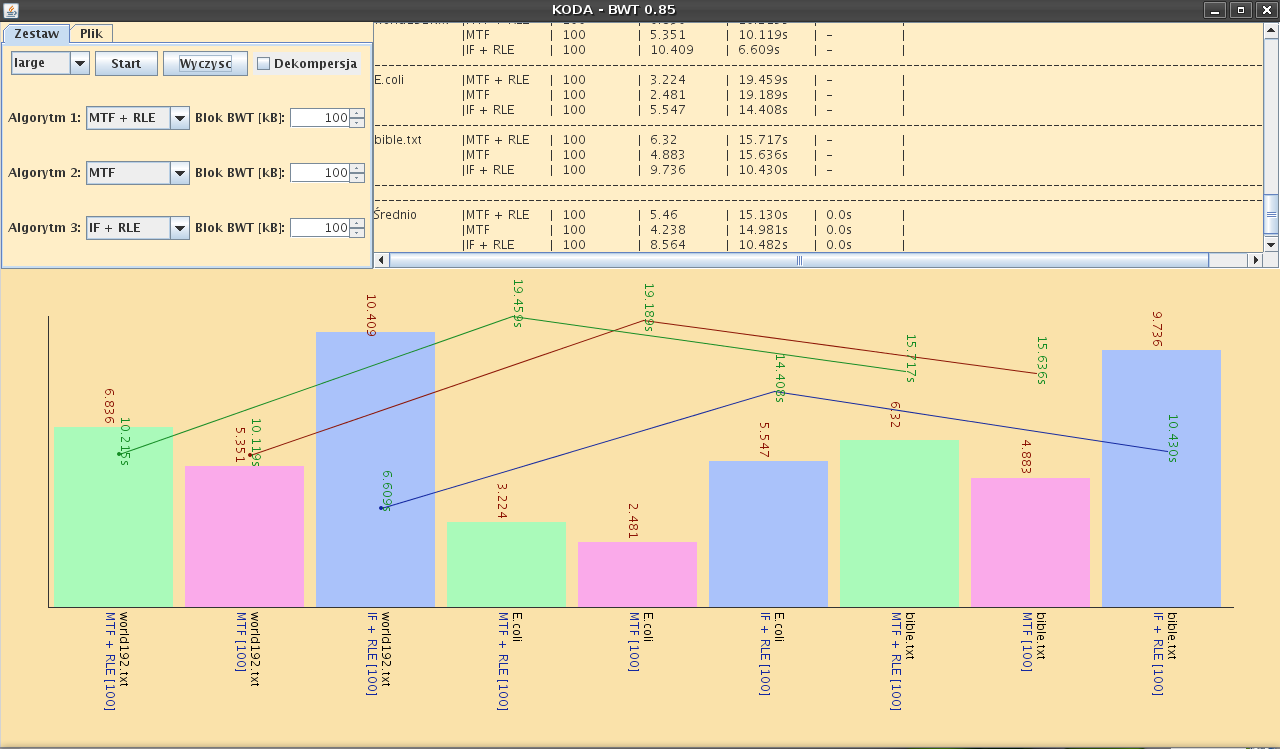
\includegraphics[scale=0.35]{\PICSDIR/test.png}
\caption{\label{fig:aplikacja_testujaca}Ekran główny aplikacji testującej}
\end{figure}